\documentclass[12pt]{article}
\usepackage{hyperref}
\usepackage[authoryear, round,sort,comma,numbers]{natbib}
\usepackage{times}
\usepackage{color}
\usepackage{apalike}
\usepackage{graphicx}
\usepackage{authblk}
\usepackage{amsmath}
\usepackage[font={sf,small}]{caption}
\usepackage{amssymb}
\usepackage{float}

\newcommand{\specialcell}[2][c]{%
	\begin{tabular}[#1]{@{}c@{}}#2\end{tabular}}
\setlength{\textheight}{9.3in}
\setlength{\textwidth}{7in}
\setlength{\footskip}{0.5in}
\setlength{\topmargin}{-0.5in}
\setlength{\headheight}{0.2in}
\setlength{\headsep}{0in}
\setlength{\parindent}{1pc}
\setlength{\oddsidemargin}{-0.25in}
\setlength{\evensidemargin}{-0.25in}
\renewcommand{\baselinestretch}{1.5}


\title{The nature of decision noise in random exploration}

\author[1]{Siyu Wang}
\author[1,2]{Robert C. Wilson}


\affil[1]{Department of Psychology, University of Arizona, Tucson AZ USA}
\affil[2]{Cognitive Science Program, University of Arizona, Tucson AZ USA}


\date{\today}

\begin{document}
	\maketitle
	
	\newpage
	\begin{abstract}
	
Human decision making is inherently variable. While this variability is often seen as a sign of suboptimality behavior, recent work suggests that variability can actually be adaptive. An example arises when we must choose between exploring unknown options or exploiting options we know well. A little randomness in these `explore-exploit' decisions is remarkably effective as it encourages us to explore options we might otherwise ignore. Recent work suggests that people may actually use such `random exploration' in practice, increasing their behavioral variability when it is more valuable to explore. 
%Other work, however, suggests that variability in human behavior is not always random, and is instead driven by deterministic factors (such as repeating past actions) 
A key question is whether the variability in random exploration is actually random. That is, is random exploration driven by stochastic processes in the brain or by some unobserved deterministic process that we have failed to account for when measuring behavioral variability? By designing an explore-exploit task in which, unbeknownst to them, participants are presented with the exact same choice twice, we provide a partial answer to this question. In particular, we find evidence that at least part (IT SOUNDS HARD TO ME TO ARGUE THAT THIS NUMBER IS NOT TASK SPECIFIC. - BOB SAYS: CAN WE PUT A NUMBER ON THIS E.G. 25\%?) of the variability in `random' exploration can be accounted for by deterministic processing of the stimulus. This still leaves open the possibility that much of random exploration is truly `random,' but narrows the window of opportunity for stochastic processes to explain this behavior.
%suggests that at least some `random' exploration is not random, but leaves open the possibility that the 
%However, it is unclear whether this variability is truly random
%From a modeling perspective, behavioral variability is essentially the variance that can not be explained by a model and is modeled as the level of decision noise. However, what we have called "decision noise" in previous researches could actually just be missing deterministic components from the model, it is difficult to tell whether decision noise truly arises from a stochastic process. Here we show that, while both random and deterministic noise drive variability in behavior, the noise driving random exploration is predominantly random. This suggests that random exploration depends on adaptive noise processes in the brain which are subject to cognitive control.

\end{abstract}
	\newpage
	\section*{Introduction}
	
	%BOB SAYS: IN GENERAL, NEED TO GO THROUGH THE PAPER AND MAKE SURE THAT `RANDOM' NOISE IS REPLACES WITH `NOT A DETERMINISTIC FUNCTION OF THE STIMULUS' OR SOMETHING LIKE THAT
	
	%(BOB SAYS: TAKE OR LEAVE THIS CHANGE TO DATE, BUT SETTING UP AS A DATE ALLOWS YOU TO TALK ABOUT AVOID YOUR EX LATER ON, WHICH MAY BE A BETTER EXAMPLE OF A DETERMINISTIC PROCESS!).
	Imagine trying to decide where to go to dinner on a date, you can go to your favorite restaurant, the one you both really enjoy and always go to, or you can try a new restaurant that you know nothing about. Such decisions, in which we must choose between a well-known `exploit' option and a lesser known `explore' option, are known as explore-exploit decisions.  From a theoretical perspective, making optimal explore-exploit choices, i.e. choices that maximize long-term reward, is computationally intractable in most cases \citep{eegittins74, eeBasu18}. In part because of this difficulty, there is considerable interest in how humans and animals solve the explore-exploit dilemma in practice \citep{, eeauer02,eegittins79,eekrebs78,eethompson33, eewatkins89, eebridle90,eemeyer95, eebanks97,eefrank09, eesteyvers09, eelee11, eepl12,eezhang13,eedaw06, eepl11, wilson2014}.
	
	One particularly effective strategy for solving the explore-exploit dilemma is choice randomization \citep{eethompson33, eewatkins89, eebridle90}. In this strategy, the decision process between exploration and exploitation is corrupted by `decision noise,' meaning that high value `exploit' options are not always chosen and exploratory choices are sometimes made by chance. In theory, such `random exploration,' is surprisingly effective and, if implemented correctly, can come close to optimal performance \citep{eethompson33, eebridle90, eeAgrawal11, eeChapelle11}.
	
	%A key limitation of our previous work was that the source of the decision noise used for exploration was left unknown.  In particular, due to the design of the task, we could not determine whether the adaptive decision noise that is linked to exploration arises deterministicly, in the input from the world, or is generated randomly, within the brain. 

	It has recently been shown that humans appear to use random exploration and can increase such decision noise when it is more beneficial to explore \citep{Gershman2018, wilson2014}. In one of these tasks, known as the Horizon Task, the key manipulation is the horizon condition, i.e. the number of decisions remaining for the participant to make. Increasing the horizon makes exploration more valuable as there is more time to use the information gained by exploration to maximize future rewards. For example, if you are leaving town tomorrow (short horizon), you will probably exploit the restaurant you know and love, but if you are in town for a while (long horizon), you would be more likely to explore the new restaurant. Using such a horizon manipulation we found that people's behavior is more variable in long horizons than short horizons, suggesting that they use adaptive decision noise to solve the explore-exploit dilemma \citep{wilson2014}. 
	
	One limitation of this previous work, is that it is difficult to tell whether what is measured as decision noise is truly random. That is, whether behavioral variability is due to intrinsic stochastic processes in the brain or whether it is due to deterministic processes that we simply have not observed.  For example, in the restaurant example, my usual preference for one restaurant or another may be overruled if I see an ex romantic partner going into one of them. Avoiding an ex is a deterministic process, but if we fail to take ex's presence into account as scientists modeling the decision, then over a series of such decisions where the ex is present or not, we would mistakenly attribute the ensuing `variability' in choice to randomness.
	
	%This difficulty arises in how noise is defined in these previous tasks. For example, in the Horizon Task, variability is defined as the inverse temperature parameter of a softmax choice function. 
	
	%In particular, in most cases noise is defined by fitting a softmax decision rule to behavior. 
	
	%because noise in previous work is defined as the component of the decision process that cannot be accounted for by a model. 
	%, what we have called 'noise' in previous research could actually just be some missing deterministic components from the model. Decision noise as defined in previous researches are more or less a quantification of what's not predictable by the model. 
	%For example, in the restaurant case above, if you happen to spot an old friend walking in to one of the restaurants, you may be more likely to follow them in. Such a process would be deterministic, in that it is driven by an observable stimulus, but unless a model of your behavior incorporated the presence of your friend, 
	
	%. If the model did not consider that the agent is favoring the behavior of following a friend in a deterministic way, the behavior of going to a less favorable restaurant because of a friend will appear to be `random' when it is really a deterministic effect. Hence this deterministic factor will be modeled as random decision noise. Crucially, however, this deterministic source of variability is very much in the stimulus and if you saw the same friend go into the same restaurant at a later date you might follow them again. Conversely, truly `random' noise would arise from stochastic mental processes, 
	
	%tossing a metaphorical coin in your head. Such a process would not be influenced by the friend going into the restaurant, and if you saw the same friend again, you might make a different choice. 
	
	%A key limitation of our previous work was that the source of the decision noise used for exploration was left unknown.  In particular, due to the design of the task, we could not determine whether the adaptive decision noise that is linked to exploration arises deterministicly, in the input from the world, or is generated randomly, within the brain. 

    % The idea here is behavior is less predictable in horizon 6 than horizon 1 even when all stimuli are the same.  Thus anything that deterministically depends on stimuli - i.e. most modeling effects - are ruled out as an explanation for increased noise.  In that light, what your model calls deterministic noise is that amount of variance that could be explained by deterministic effects of stimulus - i.e. modeling errors.

    %* Difficulty with measuring random exploration, how do you know something is random, previous work model
    %* Model all the deterministic factor (contribute to noise)
    %* Have repeated games
    %* Missing deterministic dependent, much smaller than non-deterministic component
    %* Stochastic process… 

	%In the restaurant case, an example of deterministic noise would be if you happen to spot an old friend walking in to one of the restaurants. Such an event is random, in that you couldn't predict it, and has the potential to alter your behavior as you're likely to follow your friend in. Crucially, however, this `randomness' is very much in the world and if you saw the same friend go into the same restaurant at a later date you might follow them  again. 

	%Conversely, random noise would arise from stochastic neural processes tossing a metaphorical coin in your head. Such a process would not be influenced by the friend going into the restaurant, and if you saw the same friend again, you might make a different choice. 
	
	
	%Previous work makes a strong case for both deterministic and random noise being relevant to behavior. For instance, deterministic, stimulus-driven noise is thought to be a much greater source of choice variability in perceptual decisions than random noise \citep{eeBrunton13}. Conversely random, neural noise is thought to drive exploratory singing behavior in song birds and the generation and control of this random noise has been linked to specific neural structures \citep{songbird2}. 
	
	In this paper, we investigate the extent to which the apparent randomness in random exploration can be explained by such deterministic processing of the stimulus. In particular, we modify the Horizon Task to have people face the exact same explore-exploit choice twice. If the decision is a purely deterministic function of the stimulus, then people's choices should be identical both times. That is, their choices should be consistent, since the stimulus is the same both times. Conversely, the more their decision is driven by other processes, including both stochastic and unobserved deterministic processes, the less consistent their behavior should be. By analyzing behavior on this task in both a model-free and model-based manner, we show that at least some of the `randomness' in random exploration must come from  deterministic processing of the stimulus.  This does not prove that random exploration is entirely deterministic or stochastic, but provides a lower bound on how much deterministic processes contribute to random exploration. This in turn sheds light on how random exploration may be implemented by amplifying the effects of task-irrelevant stimuli on choice.  
	
	%which source of noise, deterministic vs random, drives random exploration in humans in a modified version of the Horizon Task. To distinguish between the two types of noise, we had people make the exact same explore-exploit decision twice. If decision noise is purely deterministic noise, then people's choices should be identical both times, that is their choices should be consistent, since the stimulus is the same both times. Meanwhile, if decision noise is truly random their choices should be less consistent, since random noise can be different both times. By analyzing behavior on this task in both a model-free and model-based manner, we show that, while both types of noise are present in explore-exploit decisions, the variability related to random exploration is dominated by random noise. The missing deterministic component is much smaller than the non-deterministic component in random exploration.
	
	
		\section*{Methods}
	\subsection*{Participants}
	
	80 participants (ages 18-25, 37 male, 43 female) from the University of Arizona undergraduate subject pool participated in the experiment. 14 were excluded on the basis of performance, using the same exclusion criterion as in \citep{wilson2014}. In this exclusion criteria, we measured the accuracy of each participant's choices by calculating the percentage of times that a participant chose the bandit with the higher underlying mean payouts in the last choice of a long horizon game, intuitively people should figure out which bandit has a higher mean payout by the last trial and should have an accuracy measure significantly above 50\%, specifically, we computed the likelihood that the measured accuracy can be achieved driven by making a completely random choice between the two options and excluded participants with a likelihood smaller than 99.999\%, in other words, participants who didn't show an accuracy significant above chance with $p > 0.001$ were excluded in the analysis. This left 66 for the main analysis. Note that including the 14 badly performing subjects did not change the main results (Supplementary Figures 1 - 3)% MAKE AND INCLUDE REPLICAS OF ALL FIGS BUT WITH ALL SUBJECTS
	
	\subsection*{Task}
	The task was a modified version of the Horizon Task \citep{wilson2014} (Figure \ref{fig:taskfig}). In this task, participants play a set of games in which they make choices between two slot machines (one-armed bandits) that pay out rewards from different Gaussian distributions. In each game they made multiple decisions between two options. Each option paid out a random reward between 1 and 100 points sampled from a Gaussian distribution. The means of the underlying Gaussians were different for the two bandit options, remained the same within a game, but changed with each new game. One of the bandits always had a higher mean than the other. Participants were instructed to maximize the points earned over the entire task. To maximize their rewards in each game, participants need to exploit the slot machine with the highest mean, but they cannot identify this best option without exploring both options first. 
	
		\begin{figure}[hp]
		\begin{center}
			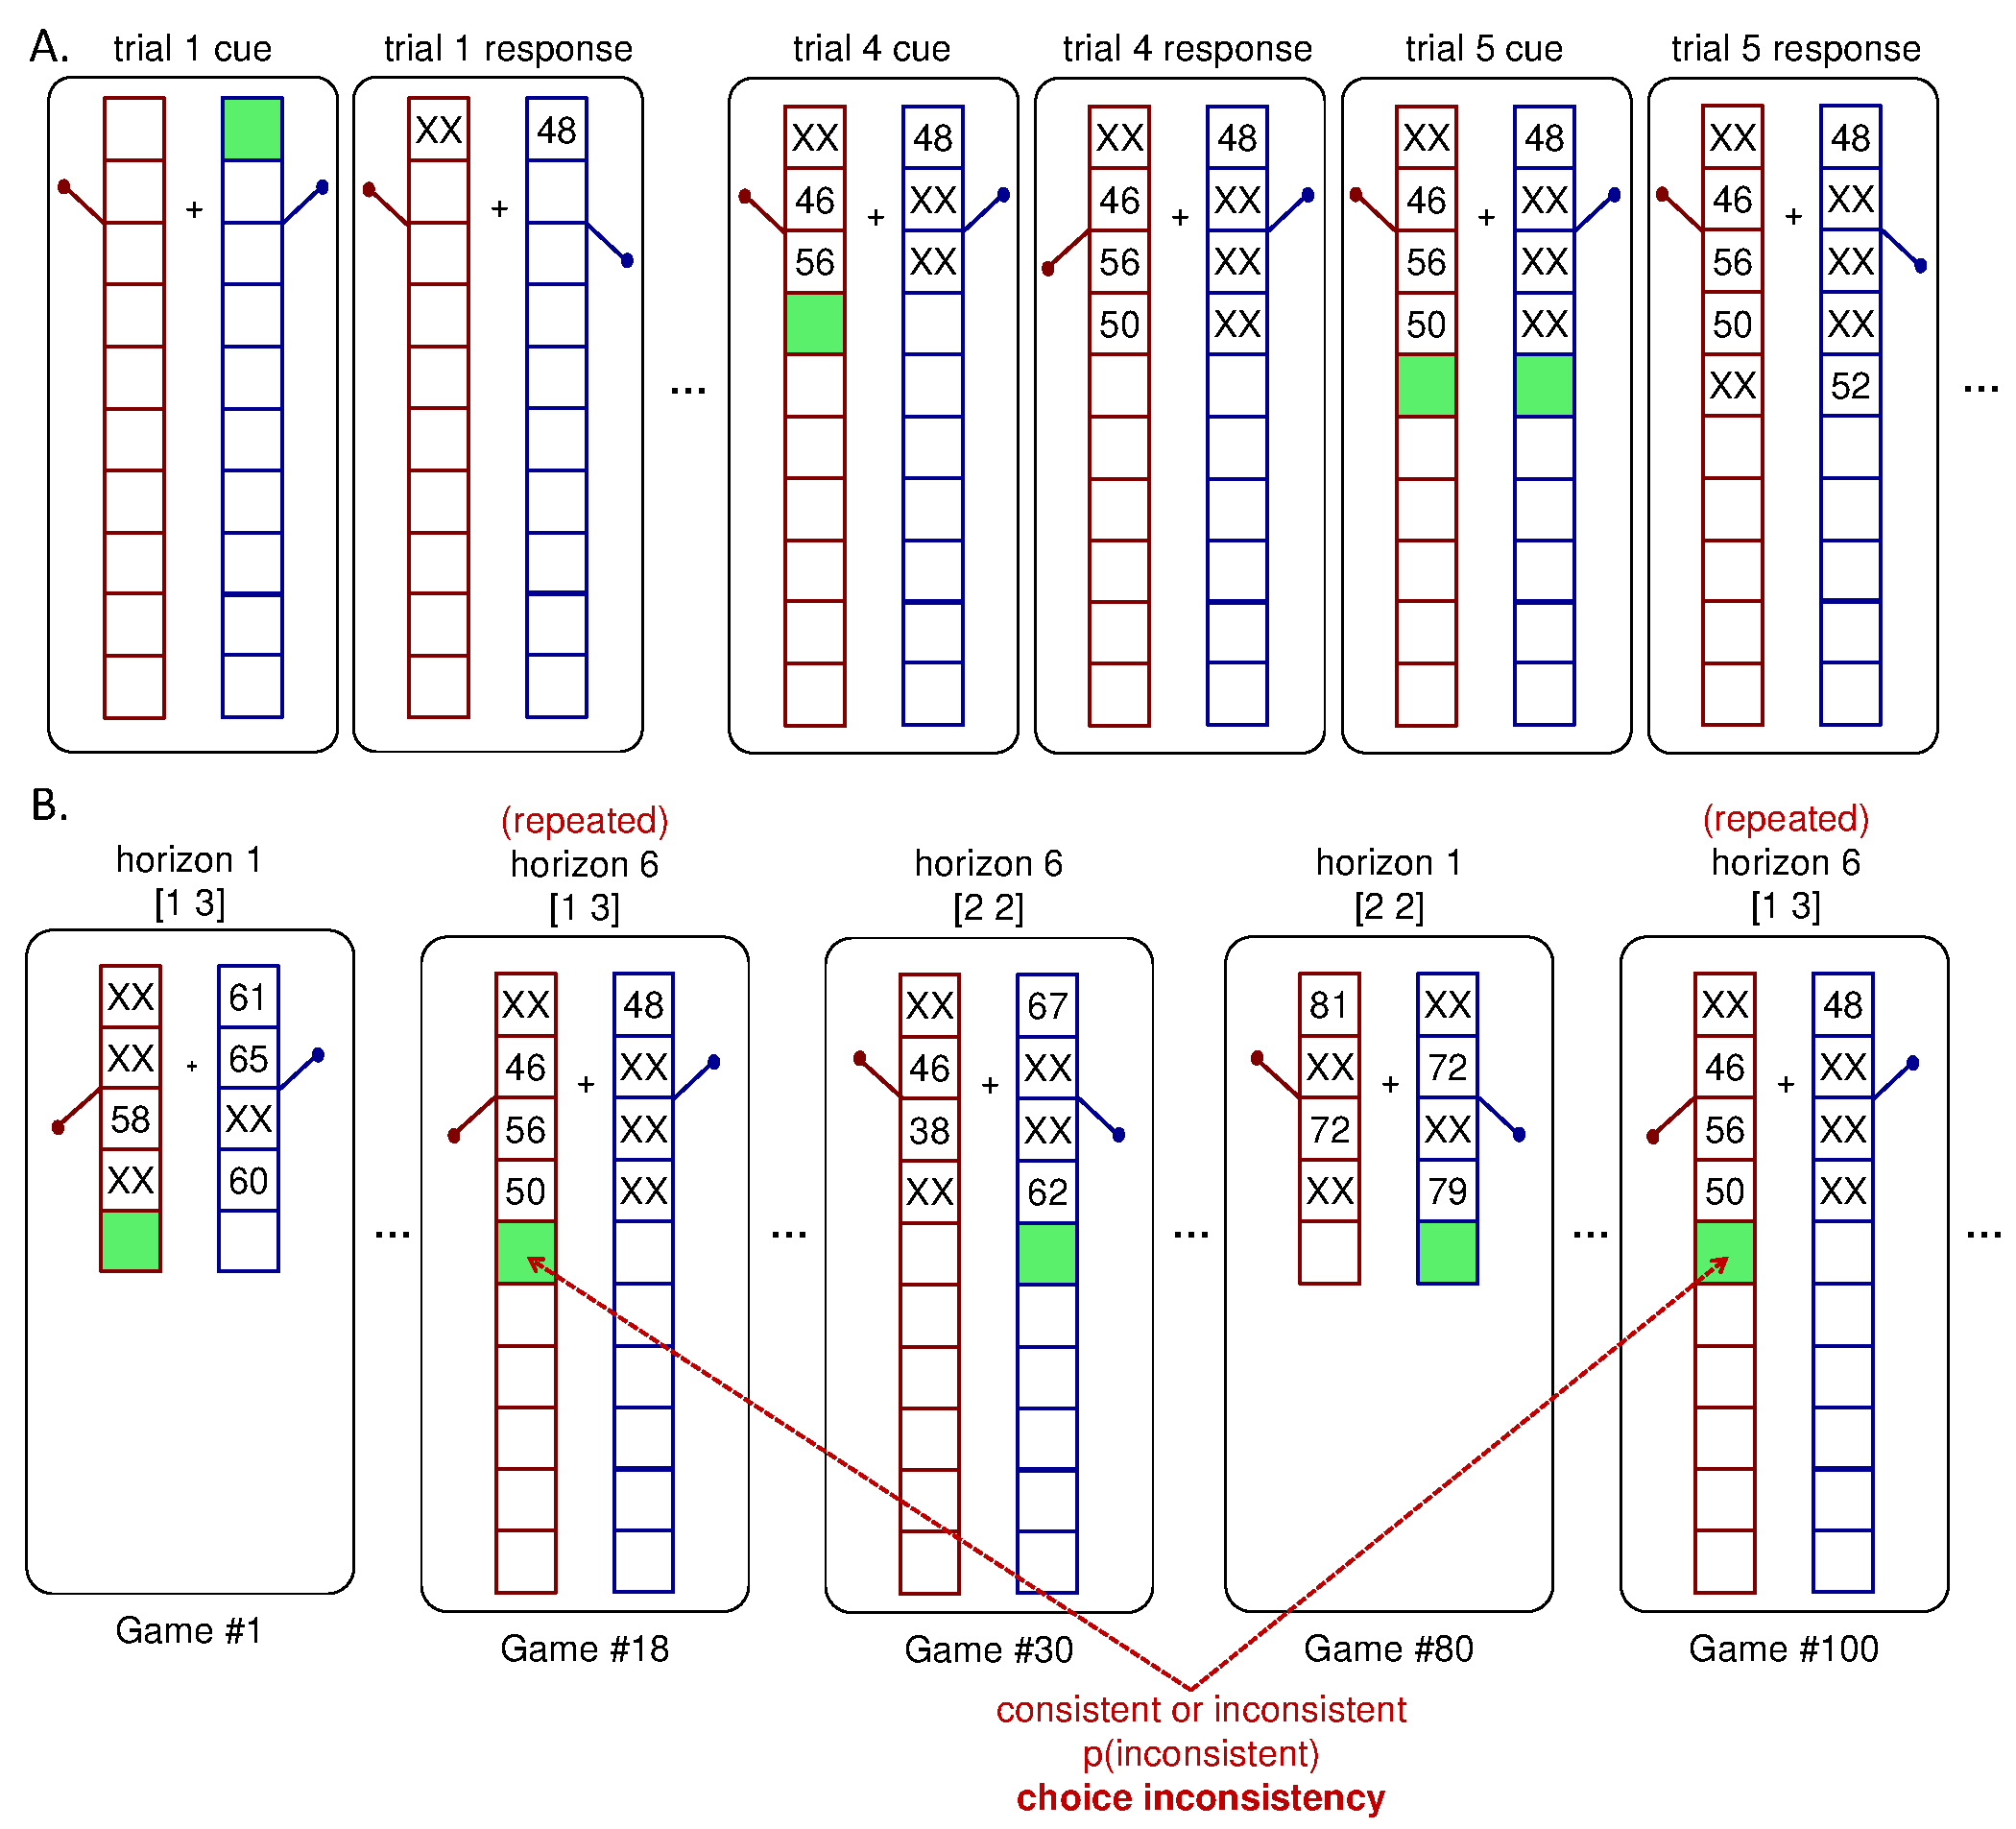
\includegraphics[width=\textwidth]{figures/taskfiga.pdf}
			\caption{ 
			Schematic of the experiment. (A) Dynamics of an example horizon 6 game.  Here the first four trials are forced trials in which participants are instructed which option to play.  After the forced trials, participants are free to choose between the two options for the remainder of the game.  (B) Different possible states of the game after the first free choice over the course of the experiment. Overall participants play 160 such games, with varying horizon (1 vs 6), uncertainty condition ([1 3] vs [2 2]) and observed rewards.  In addition, all games are repeated (as Game 18 and 100 are here) such that participants will be faced with the exact same pattern of forced trials and exact same outcomes from those forced trials twice within each experiment.  These repeated games allow us to compute the relative contribution of deterministic and random noise by analyzing the extent to which choices are {\em consistent} across the repeated games.}
			\label{fig:taskfig}
		\end{center}
	\end{figure}
	
	
	The number of games participants played depended on how well they performed, which acted as the primary incentive for performing the task. Thus, the better participants performed, the sooner they got to leave the experiment. On average, participants played 151.6 games (minimum = 90 games, maximum = 192 games) and the whole task lasted between 12.34 and 32.74 minutes (mean 23.31 minutes). Participants played an average of 67.31 repeated pairs of games (minimum = 25 repeated pairs, maximum =  100 repeated pairs).
	%BOB SAYS: ADD HOW MANY REPEATED GAMES THEY PLAYED - GIVE A MEAN AND RANGE FOR THIS NUMBER
	
	As in the original paper \citep{wilson2014}, the distributions of payoffs tied to bandits were independent between games and drawn from a Gaussian distribution with variable means and fixed standard deviation of 8 points. Differences between the mean payouts of the two slot machines were set to either 4, 8, 12 or 20. One of the means was always equal to either 40 or 60 and the second was set accordingly. Participants were informed that in every game one of the bandits always has a higher mean reward than the other. The order of games was randomized. Mean sizes and order of presentation were counterbalanced. 
	
	Each game consisted of 5 or 10 choices. Every game started with a fixation cross, then a bar of boxes appeared indicating the horizon for that game. For the first 4 trials - the instructed trials, we highlight the box on one of the bandits to instruct the participant to choose that option. On these trials, they have to press the corresponding key to reveal the outcome. From the fifth trial, boxes on both bandits will be highlighted and they are free to make their own decision. There was no time limit for decisions. During free choices participants could press either the left arrow key or right arrow key to indicate their choice of left or right bandit. The score feedback was presented for 300ms. The task was programmed using Psychtoolbox in MATLAB \citep{psychtoolbox1, psychtoolbox2}. 
	
	The first four trials of each game were forced-choice trials, in which only one of the options was available for the participant to choose. We used these forced-choice trials to manipulate the relative ambiguity of the two options, by providing the participant with different amounts of information about each bandit before their first free choice. The four forced-choice trials set up two uncertainty conditions: unequal uncertainty(or [1 3]) in which one option was forced to be played once and the other three times, and equal uncertainty(or [2 2]) in which each option was forced to be played twice. After the forced-choice trials, participants made either 1 or 6 free choices (two horizon conditions),  Figure \ref{fig:taskfig}.
	
	\subsection*{Model-based analysis}
	We modeled behavior on the first free choice of the Horizon Task using a version of the logistic choice model in \citep{wilson2014} that was modified to differentiate between components of the noise that are deterministically driven by the stimulus (`deterministic noise') and components of the noise that are not deterministically driven by the stimulus (`random noise').  Because the stimuli are identical in the repeated games, by definition, deterministic noise remains the same in repeated games, whereas random noise can change. 
	
	\subsubsection*{Hierarchical Bayesian Model}
	
	To model participants' choices on this first free-choice trial, we assume that they make decisions by computing the difference in value $\Delta Q$ between the right and left options, choosing right when $\Delta Q > 0$ and left otherwise.  Specifically, we write
	\begin{equation}
	\Delta Q= \Delta R+A \Delta I+b+n_{det}+n_{ran}
	\end{equation}
	where, the experimentally controlled variables are $\Delta R=R_{right}-R_{left}$, the difference between the mean of the rewards shown on the forced trials, and $\Delta I$, the difference information available for playing the two options on the first free-choice trial. For simplicity, and because information is manipulated categorically in the Horizon Task, we define $\Delta I$ to be +1, -1 or 0, +1 if one reward is drawn from the right option and three are drawn from the left in the [1 3] condition, -1 if one from the left and three from the right, and in [2 2] condition, $\Delta I$ is 0. $n_{det}$ and $n_{ran}$ are deterministic noise and random noise respectively. 
	
	The other variables are: the spatial bias, $b$, which determines the extent to which participants prefer the option on the right; the information bonus $A$, which controls the level of directed exploration; $n_{det}$ denotes the deterministic noise, which is identical on the repeat versions of each game; and $n_{ran}$ denotes random noise, which is uncorrelated between repeat plays and changes every game.
	
	Each subject's behavior in each horizon condition is described by 4 free parameters: the information bonus $A$, the spatial bias, $b$, the standard deviation of the deterministic noise, $\sigma_{det}$, and the standard deviation of the random noise, $\sigma_{ran}$ (Table \ref{tab:pars2}, Figure \ref{fig:model}). Each of the free parameters is fit to the behavior of each subject using a hierarchical Bayesian approach \citep{hbm1}.  In this approach to model fitting, each parameter for each subject is assumed to be sampled from a group-level prior distribution whose parameters, the so-called `hyperparameters', are estimated using a Markov Chain Monte Carlo (MCMC) sampling procedure. The hyper-parameters themselves are assumed to be sampled from `hyperprior' distributions whose parameters are defined such that these hyperpriors are broad.  
	
	The particular priors and hyperpriors for each parameter are shown in Table \ref{tab:pars2}. For example, we assume that the information bonus, $A^{is}$, for each horizon condition $i$ and for each participant $s$, is sampled from a Gaussian prior with mean $\mu^{A}_{i}$ and standard deviation $\sigma_{i}^A$. These prior parameters are sampled in turn from their respective hyperpriors: $\mu_{i}^{A}$, from a Gaussian distribution with mean 0 and standard deviation 10, and $\sigma_{i}^A$ from an Exponential distribution with parameters 0.1.
	
	\begin{table}[h]
		\small
		\begin{tabular}{|c|c|c|c|}
			\hline
			Parameter & Prior & Hyperparameters & Hyperpriors \\
			\hline
			information bonus, $A_{is}$ 
			& $A_{is} \sim $  Gaussian($\mu_i^{A}$, $\sigma_i^{A}$) 
			& $\theta_{i}^{A} = (\mu_i^{A}, \sigma_i^{A}) $
			& \specialcell{
				$\mu_i^{A} \sim $ Gaussian( 0, 100 ) \\ 
				$\sigma_i^{A} \sim $ Exponential(0.01)}		\\
			\hline
			spatial bias, $b_{is}$ 
			& $b_{is} \sim $  Gaussian($\mu_i^{b}$, $\sigma_i^{b}$) 
			& $\theta_{i}^{b} = (\mu_i^{b}, \sigma_i^{b}) $
			& \specialcell{
				$\mu_i^{b} \sim $ Gaussian( 0, 100 ) \\ 
				$\sigma_i^{b} \sim $ Exponential(0.01)}		\\
			\hline
			deviation of deterministic noise, $\sigma^{det}_{isg}$ 
			& $\sigma_{i} \sim $  Gamma($k_i^{det}$, $\lambda_{i}^{det}$) 
			& $\theta_{i}^{det} = (k_i^{det}, \lambda_i^{det}) $
			& \specialcell{
				$k_i^{det} \sim $ Exponential(0.01) \\ 
				$\lambda_i^{det} \sim $ Exponential(10)}		\\
			\hline
			deviation of random noise, $\sigma^{ran}_{isgr}$ 
			& $\sigma_{is} \sim $  Gamma($k_i^{ran}$, $\lambda_{i}^{ran}$) 
			& $\theta_{i}^{ran} = (k_i^{ran}, \lambda_i^{ran}) $
			& \specialcell{
				$k_i^{ran} \sim $ Exponential(0.01) \\ 
				$\lambda_i^{ran} \sim $ Exponential(10)}		\\
			\hline
		\end{tabular}
		\caption{Model parameters, priors, hyperparameters and hyperpriors. }%CHECK UPDATE}
		\label{tab:pars2}	
	\end{table}
	
	\subsubsection*{Model fitting using MCMC}
	The model was fit to the data using Markov Chain Monte Carlo approach implemented in the JAGS package \citep{jags} via the MATJAGS interface (psiexp.ss.uci.edu/research/programs\_data/jags). This package approximates the posterior distribution over model parameters by generating samples from this posterior distribution given the observed behavioral data.  
	
	In particular we used 4 independent Markov chains to generate 16000 samples from the posterior distribution over parameters (4000 samples per chain).  Each chain had a burn in period of 2000 samples, which were discarded to reduce the effects of initial conditions, and posterior samples were acquired at a thin rate of 1.  Convergence of the Markov chains was confirmed {\it post hoc} by eye. 
	
	\begin{figure}[H]
		\begin{center}
			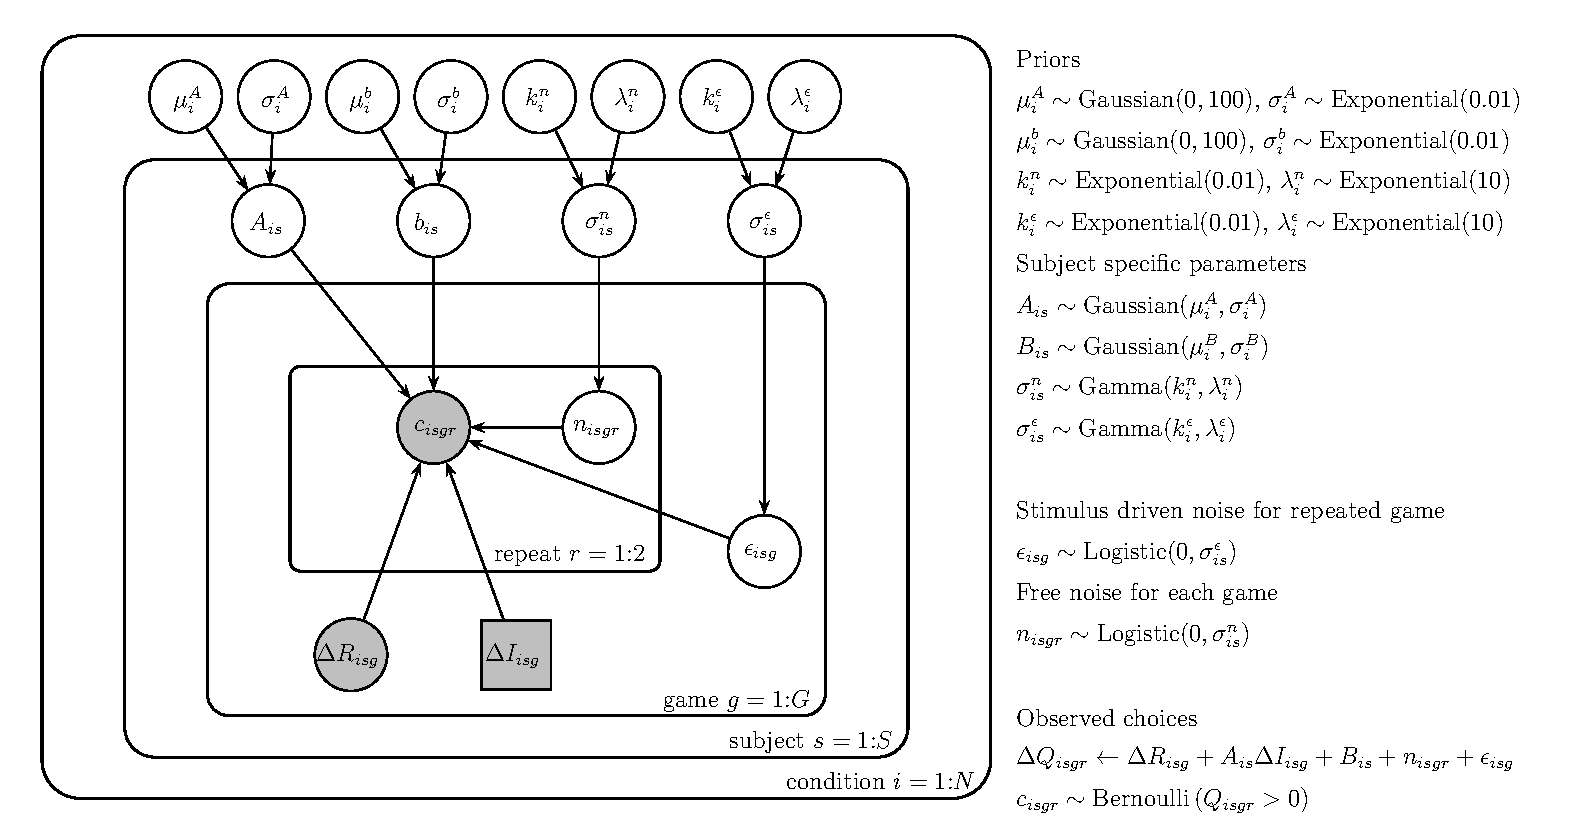
\includegraphics[width=1\textwidth]{figures/Siyu_EEHorizon_2sigma_final.pdf}
    			\caption{Schematic of the hierarchical Bayesian model using notation of \cite{lee_wagenmakers_2014}}
			\label{fig:model}
		\end{center}
	\end{figure}
	
	\subsubsection*{Parameter recovery\label{ch:appendix:bayesrecovery}}
	
	To be sure that our fit parameter values were meaningful, we tested the ability of our model fitting procedure to recovery parameters from simulated data.  In particular, we simulated choices with the fitted parameters from the Hierarchical Bayesian analysis, and the re-fit the simulated choices to see whether we can recover the parameters. 
	
	Results of this parameter recovery procedure are shown in Supplementary Figure S4. As is clear from this figure, parameter recovery is good in terms of correlation between the true vs fitted parameters for all parameters apart from the bias in short horizon condition, which is likely due to this parameter being so close to zero (Supplementary Figure S4 Panel C). The recovery for the noise parameters, $\sigma_{det}$ and $\sigma_{ran}$, is slightly better for horizon 1 than horizon 6. This is because it requires more trials to recover bigger noises, so with the same number of choices it is harder to recover overall bigger noises in horizon 6. In addition we see better recovery for random noise than deterministic noise because we effectively have half as many trials for deterministic noise since we are only generating one sample of deterministic noise for each repeated game pair. 
	
	One limitation of our model is that we observed a systematic underestimation of deterministic noise (despite the strong correlation). This is further illustrated in Supplementary Figure S5. In thee simulation with 0 random noise and full deterministic noise, our model perfectly recovered both random and deterministic noise, however in the simulation with full random noise and 0 deterministic noise, our model recovered only XXX \% of deterministic noise, and the remaining shows up as random noise instead (See Supplementary Figure S5). Thus, our model provides a lower bound on deterministic noise and an upper bound on random noise.
	
	Overall, we are able to recover both deterministic and random noises using our model to a satisfactory extent.
	
	\subsection*{Data and code}
	Behavioral data as well as Matlab code to recreate the main figures from this paper will be made available on the Dataverse website upon publication. %website at https://dataverse.harvard.edu/dataset.xhtml?persistentId=doi:10.7910/DVN/CZT6EE.
	
	\section*{Results}
	
	\subsection*{The Repeated-Games Horizon Task}
	We used a modified version of the `Horizon Task' \citep{wilson2014} to show the influence of stimulus-driven `deterministic noise' vs non-stimulus driven `random noise' on people's decisions (Figure \ref{fig:taskfig}). In this task, participants make repeated choices between two slot machines, or `one-armed bandits,' that pay out probabilistic rewards. Because they are initially unsure as to the mean payoff of each bandit, this task requires that participants carefully balance exploration of the lesser known bandit with exploitation of the better known bandit to maximize their overall rewards. 
	
	Crucially, before people make their first choice in the Horizon Task, they are given information about the mean payoff from each bandit in the form of four example plays distributed either unequally between bandits (i.e. 1 play of one bandit, 3 plays of the other, the [1 3] condition) or equally (2 plays each, the [2 2] condition). These example plays allow us to manipulate exactly what people know about each option before they make their first choice. 
	
	Relative to the original Horizon Task, the key modification here is to give people `repeated games,' in which they see exact same set of example plays twice in two separate games (separated by several minutes in time so as to avoid detection). By repeating the instructed plays for each game twice, we can set up a situation where (unbeknownst to the participants) they are faced with the exact same explore-exploit choice, with the exact same stimuli twice. Thus, if their behavior is a deterministic function of the stimuli, they will behave identically on the two games, that is their behavior on the two versions of each game will be consistent. Conversely, if their behavior is not driven by a deterministic function of the stimulus, then their choices on the repeated games should be inconsistent.
	
	On average participants played 67.31 repeated games each allowing us to quantify the extent to which their behavior was a deterministic function of the stimulus or not.
	
	%, the example plays allow us to probe how participants respond to the exact same explore-exploit choice twice.  
	
	%These `repeated games' are the key manipulation in this paper and allow us to distinguish between deterministic and random sources of noise.  Specifically, if noise is deterministicly driven, then choices on repeated games should be consistent. Conversely if noise is randomly driven, then choices on repeated games should be inconsistent.
	

	\subsection*{Both behavioral variability and information seeking increase with horizon}
	
	Before discussing the results for repeated games, we first confirm that the basic behavior in this task is consistent with our previously reported results \citep{wilson2014}. As in our previous work, we find evidence for two types of exploration in the Horizon Task.  Random exploration, which is the main focus of this paper, where exploration is driven by noise, and directed exploration, where exploration is driven by information. 
	
	Random exploration is quantified in a model-free way as the probability of choosing the low mean option, $p(\mbox{low mean})$ in the equal, or [2 2], condition. This value increases with horizon, consistent with the idea that behavior is more random in horizon 6 (t(65) = 6.60, p $<$ 0.001 for [1 3], t(65) = 8.14, p $<$ 0.001 for [2 2]).  Directed exploration, is measured as the probability of choosing the more informative option $p(\mbox{high info}$ in the unequal, or [1 3], condition. Again this measure increases with horizon, showing that people are more information seeking in horizon 6 (t(65) = 7.00, p $<$ 0.001).
	
	\begin{figure}[H]
		\begin{center}
			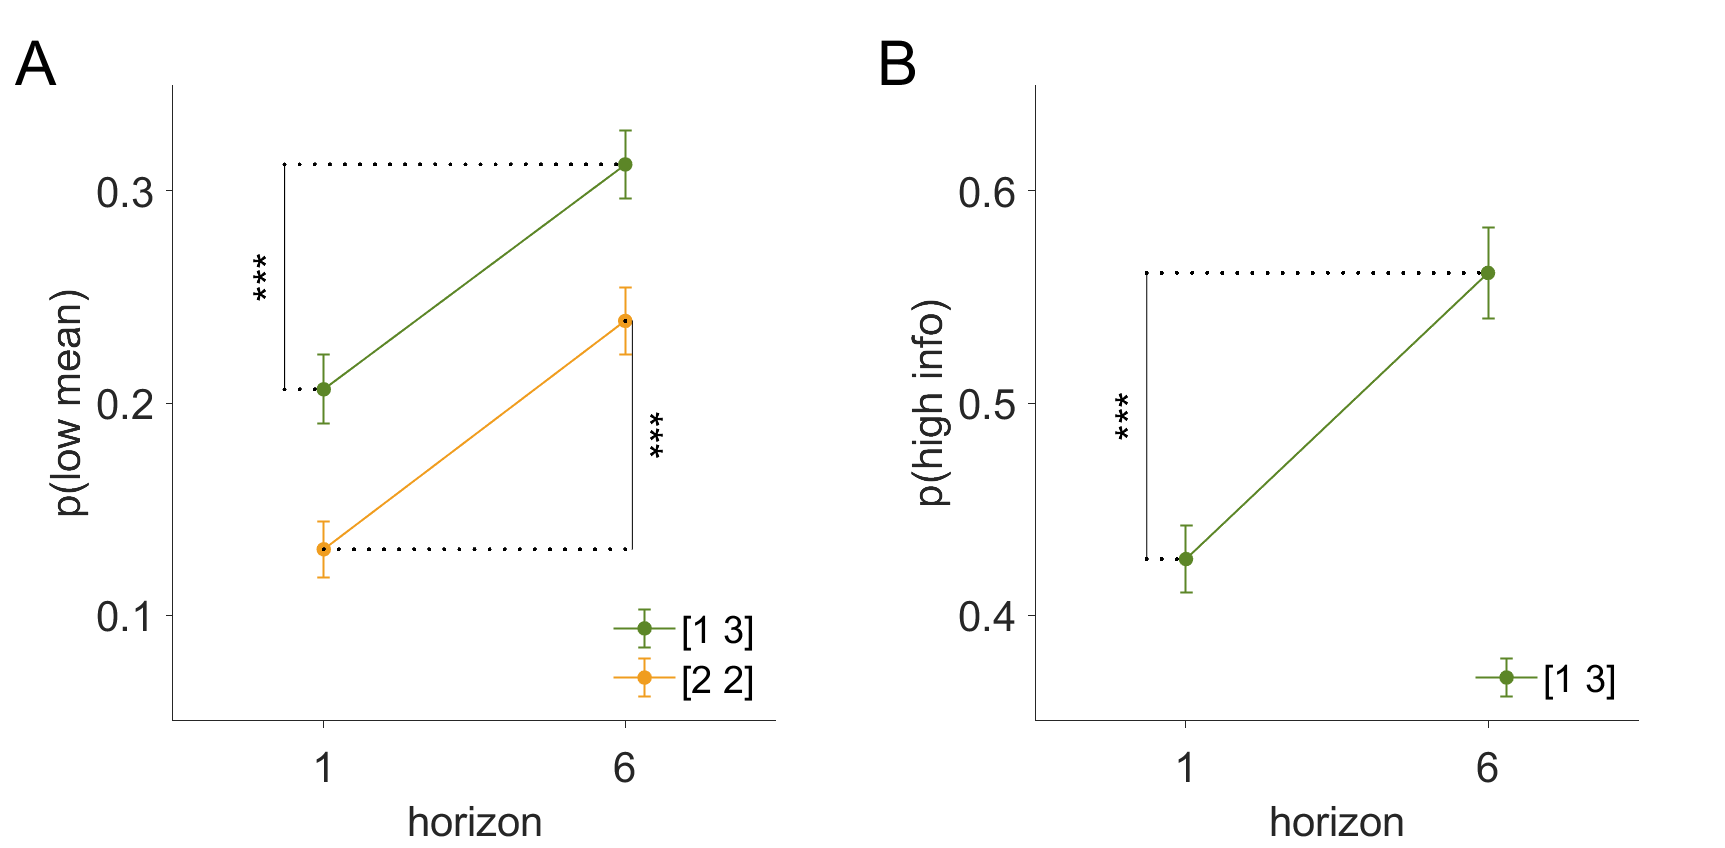
\includegraphics[width=\textwidth]{figures/line_modelfree.png}
			\caption{
			Replication of previous findings. Both  $p(\mbox{low mean})$ (A) and $p(\mbox{high info})$ (B) increase with horizon suggesting that people use both random and directed exploration in this task.  }
			\label{fig:modelfree}
		\end{center}
	\end{figure}
	
	\subsection*{Model-free analysis shows that random exploration may involve both random and deterministic noise}
	
	Next we asked whether participants' choices were consistent or inconsistent in the two repetitions of each game.  The idea behind this measure is that purely deterministic noise should lead to consistent choices as the deterministic stimulus is identical both times. Conversely, if choice is not a deterministic function of the stimulus, participants' choices should be independent, and hence more inconsistent across the repetitions of the game. 
	
	To quantify choice inconsistency we computed the frequency with which participants made different responses for pairs of repeated games (Figure \ref{fig:mf2}). Using this measure we found that participants made inconsistent choices in both the unequal ([1 3]) and equal ([2 2]) information conditions, suggesting that not all of the noise was stimulus driven (t-test vs zero revealed that inconsistency was greater than zero for all horizon and uncertainty conditions.  For [1 3] condition, t(65) = 12.92, p $<$ 0.001 for horizon 1, t(65) = 16.76, p $<$ 0.001 for horizon 6; For [2 2] condition, t(65) = 9.67, p $<$ 0.001 for horizon 1, t(65) = 17.74, p $<$ 0.001 for horizon 6). In addition, we found that choice inconsistency was higher in horizon 6 than in horizon 1 for both [1 3] and [2 2] condition (F(1, 196) = 61.19, p $<$ 0.001), suggesting that at least some of the horizon dependent noise is not a deterministic function of the stimulus.
	
	\begin{figure}[h]
		\begin{center}
			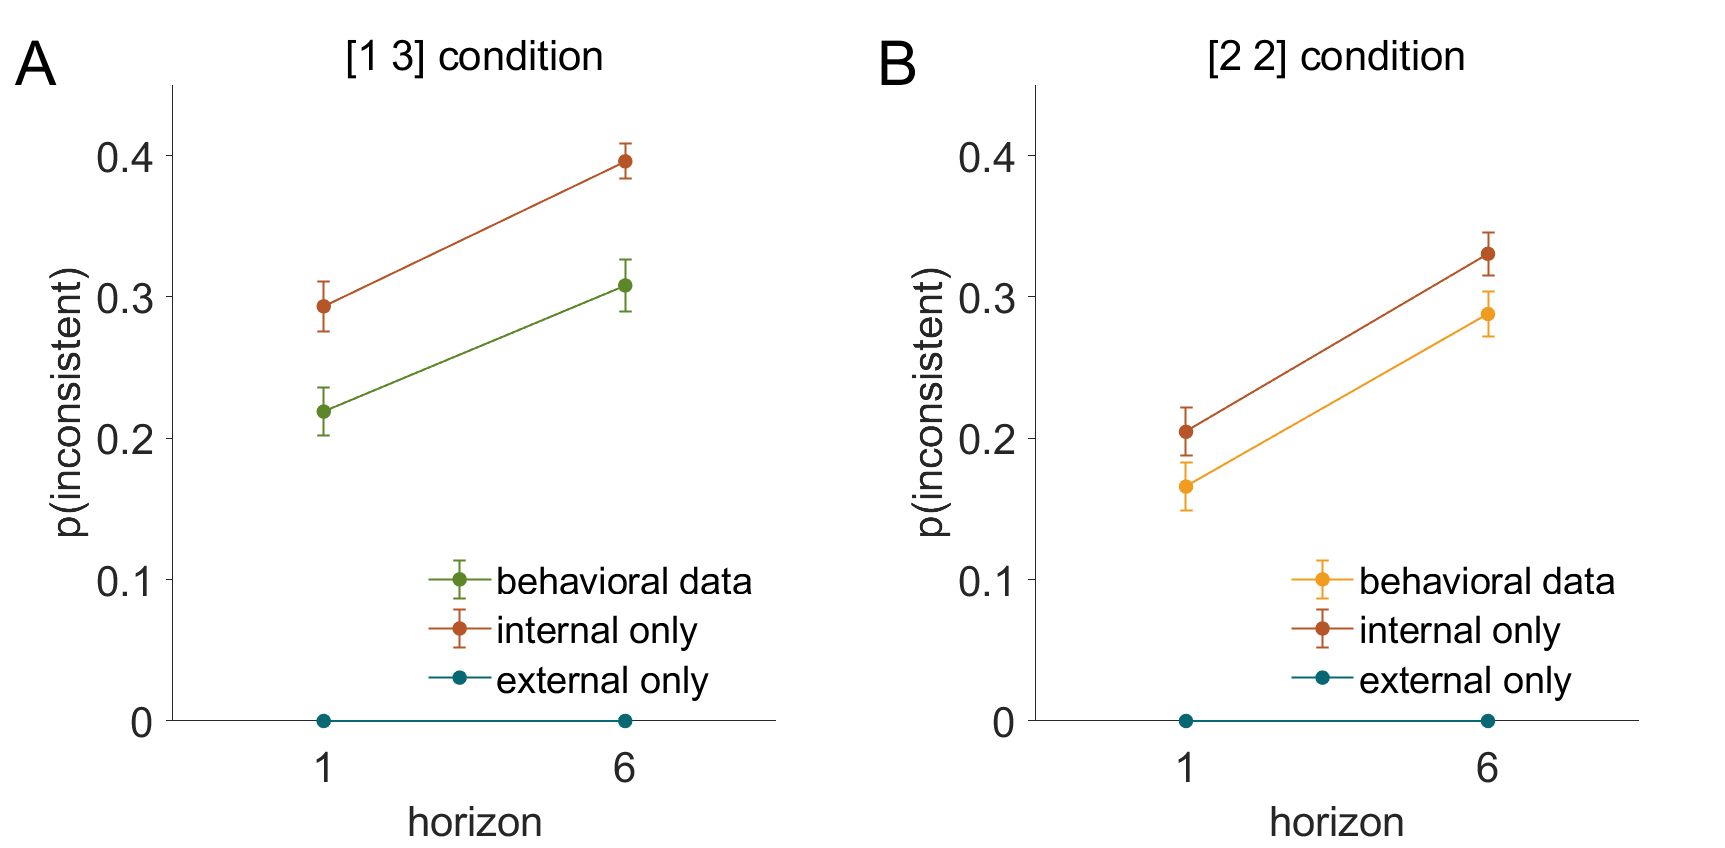
\includegraphics[width=\textwidth]{figures/theory_da_info.png}
			\caption{Model-free analysis suggests that both deterministic and random noise contribute to the choice variability in random exploration. For both the [1 3] (A) and [2 2] (B) condition, people show greater choice inconsistency in horizon 6 than horizon 1. However, the extent to which their choices are inconsistent lies between what is predicted by purely deterministic and random noise, suggesting that both noise sources influence the decision.}
			\label{fig:mf2}
		\end{center}
	\end{figure}
	
	To gain more quantitative insight into these results, we computed theoretical values for the choice inconsistency for the purely deterministic and purely random noise cases.  For purely deterministic noise this computation is simple because people should make the exact same decisions each time in repeated games, meaning that $p(\mbox{inconsistent}) = 0$ in this case. For purely random noise, the two games should be treated independently, allowing us to compute the choice inconsistency in terms of the probability of choosing the low mean option, $p(\mbox{low mean})$, as
	\begin{equation*}
	\begin{split}
	p(\mbox{consistent}) &= p(\mbox{low mean})^2 + p(\mbox{high mean})^2\\
	&= p(\mbox{low mean})^2 + (1-p(\mbox{low mean}))^2\\ 
	\mbox{hence},\quad p(\mbox{inconsistent}) &=  
	1 - p(\mbox{consistent}) = 
	2 p(\mbox{low mean})(1-p(\mbox{low mean}))
	\end{split}
	\end{equation*}
	As shown in Figure  \ref{fig:mf2}, people's behavior falls in between the pure deterministic noise prediction and the pure random noise prediction Specifically, behavior is different from pure random noise prediction in the both the [1 3] condition (t(65) = 5.60, p $<$ 0.001 for horizon 1, t(65) = 5.62 p $<$ 0.001 for horizon 6) and [2 2] condition (t(65) = 3.86, p $<$ 0.001 for horizon 1, t(65) = 3.42, p $<$ 0.001 for horizon 6). Likewise, behavior is different from pure deterministic noise prediction in both the [1 3] condition ( t(65) = 12.92, p $<$ 0.001 for horizon 1, t(65) = 16.76, p $<$ 0.001 for horizon 6) and the [2 2] condition (t(65) = 9.67, p $<$ 0.001 for horizon 1, t(65) = 17.74, p $<$ 0.001 for horizon 6). This suggests that at least some of the `noise' is a deterministic function of the stimulus, although from this analysis it is not clear whether this deterministic noise increases with horizon or not.
	
	\subsection*{Model-based analysis shows deterministic noise changes with horizon}
	
	To more precisely quantify the contribution of stimulus-driven deterministic noise, we turned to model fitting. We modeled behavior on the first free choice of the Horizon Task using a version of the logistic choice model in \citep{wilson2014} that was modified to differentiate deterministic noise from and random noise. In particular, we assume that in repeated games, the value of stimulus-driven deterministic noise is frozen whereas random noise is drawn independently both times. 
	
	\subsubsection*{Overview of model}
	As with our model-free analysis, the model-based analysis focuses only on the first free-choice trial since that is the only free choice when we have control over the experience participants have about two bandits. To model participants' choices on this first free-choice trial, we assume that they make decisions by computing the difference in value $\Delta Q$ between the right and left options, choosing right when $\Delta Q > 0$ and left otherwise.  Specifically, we write
	\begin{equation}
	\Delta Q= \Delta R+A \Delta I+b+n_{det}+n_{ran}
	\end{equation}
	where, the experimentally controlled variables are $\Delta R=R_{right}-R_{left}$, the difference between the mean of rewards shown on the forced trials, and $\Delta I$, the difference information available for playing the two options on the first free-choice trial. For simplicity, and because information is manipulated categorically in the Horizon Task, we define $\Delta I$ to be +1 if one reward is drawn from the right option and three are drawn from the left in the [1 3] condition, -1 if one from the left and three from the right, and in [2 2] condition, $\Delta I$ is 0. $n_{det}$ and $n_{ran}$ are deterministic noise and random noise respectively which are assumed to come from logistic distributions with mean 0.
	
	The subject-and-condition-specific parameters are: the spatial bias, $b$, which determines the extent to which participants prefer the option on the right; the information bonus $A$, which controls the level of directed exploration; $n_{det}$ denotes the deterministic noise, which is identical on the repeat versions of each game; and $n_{ran}$ denotes random noise, which is uncorrelated between repeat plays and changes every game.
	
	For each pair of repeated games, the set of forced-choice trials are exactly the same, so the deterministic noise, $n_{det}$, should be the same while the random noise, $n_{ran}$ may be different. This is exactly how we distinguish deterministic noise from random noise. In symbolic terms, for repeated games $i$ and $j$,  $n_{det}^i=n_{det}^j$  and $n_{ran}^i \neq n_{ran}^j$.
	
	
	\subsubsection*{Model fitting}
	We used hierarchical Bayesian analysis to fit the parameters of the model (see Figure \ref{fig:model} for an graphical representation of the model in the style of \cite{lee2014}). In particular, we fit values of the information bonus $A$, spatial bias $B$, variance of random noise $\sigma_{ran}^2$, and variance of deterministic noise, $\sigma_{det}^2$ for each participant in each horizon. Model fitting was performed using the MATJAGS and JAGS software \citep{jags, matjags} with full details given in the Methods.  
	
	\subsubsection*{Model fitting results} 
	
	Posterior distributions over the group-level means of the deterministic and random noise variance are shown in Figure \ref{fig:mb1}. Consistent with our model-free results, we see that both random and deterministic noise variances are non-zero and that random noise is about 2-3 times larger than the deterministic noise. In addition, we find that both random and deterministic noise increase with horizon.  This increase was larger for random noise (M = 4.55, 100\% of samples showed an increase in random noise with horizon) than deterministic noise (M = 1.78, 98.12\% of samples showed an increase in deterministic noise with horizon). But intriguingly the relative increase in both types of noise was the same (Figure \ref{fig:ratio}). That is when we compute the relative increase in deterministic noise with horizon, $\sigma_{det, horizon6}/\sigma_{det, horizon1}$, it is almost identical to the relative increase in random noise with horizon $\sigma_{ran, horizon6}/\sigma_{ran, horizon1}$. 
	%BOB SAYS: CHECK NOTATION HERE AND INSERT FIGURE SHOWING RATIO  
	
	
	\begin{figure}[hp]
		\begin{center}
			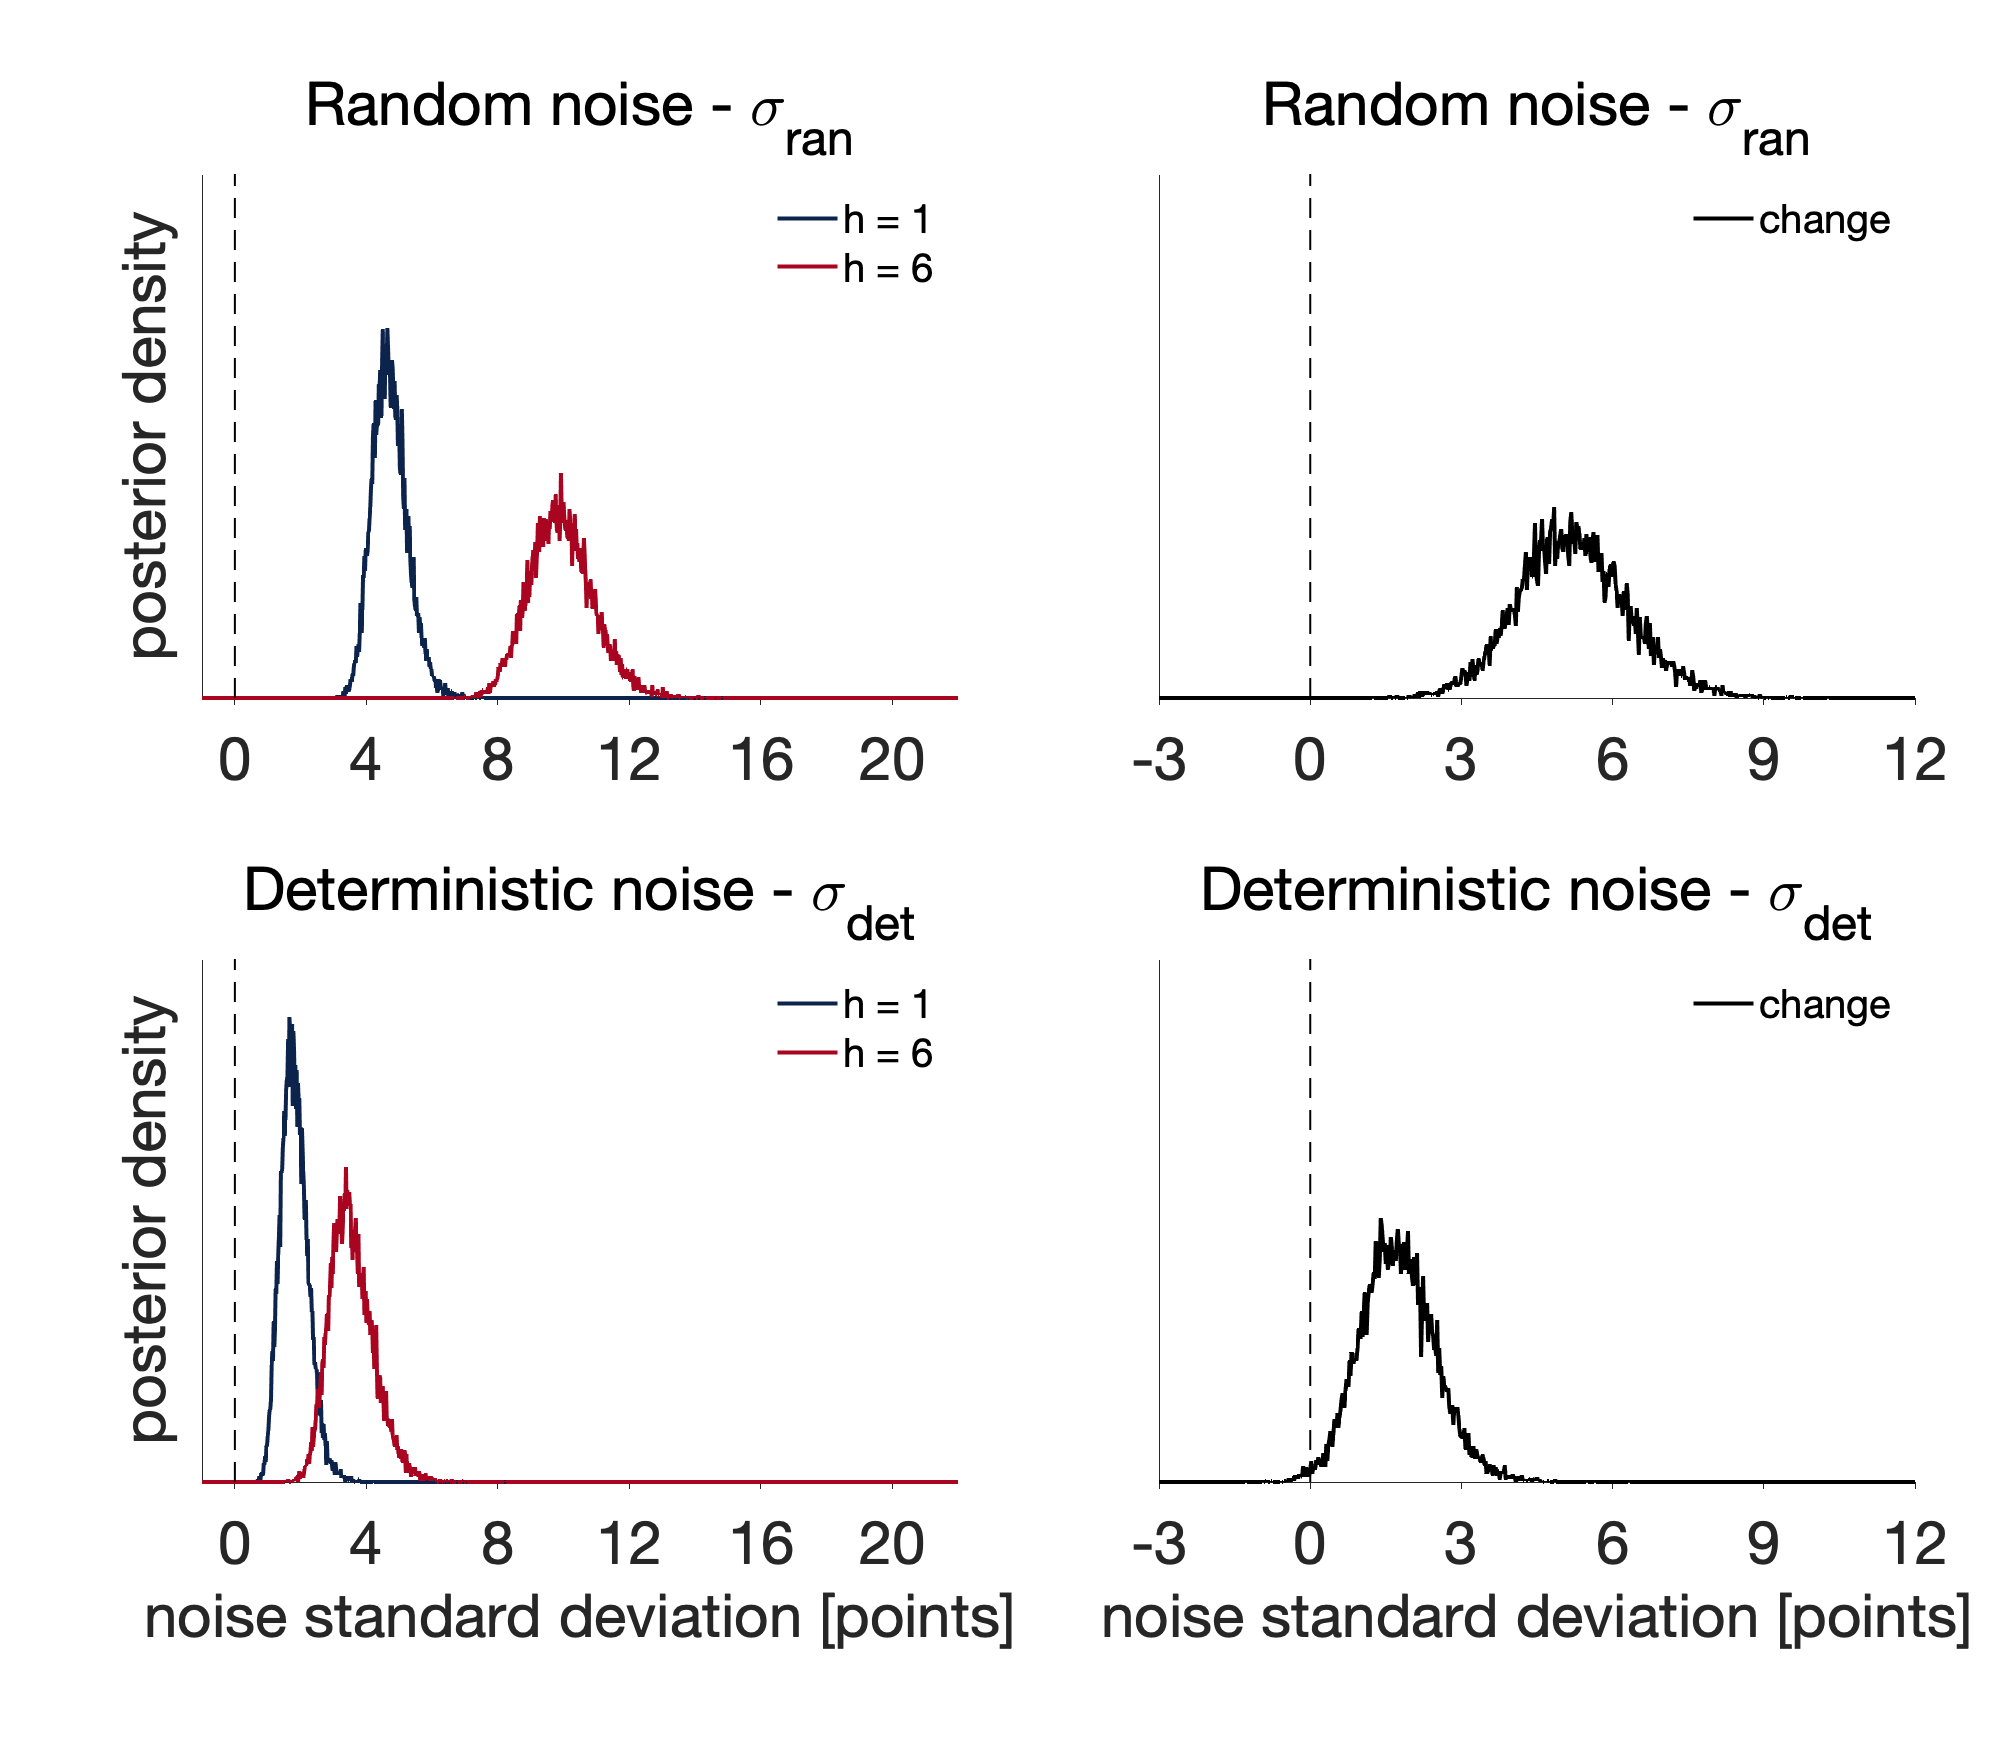
\includegraphics[width=1\textwidth]{figures/hyperprior.png}
			\caption{Model based analysis showing the posterior distributions over the group-level mean of the standard deviations of  random and deterministic noise. Both random (A, B) and deterministic (C,D) noises are nonzero (A, C) and change with horizon (B, D).  However, random noise has both a greater magnitude overall (A, C) and a greater change with horizon (B, D) than deterministic noise.}
			%BOB SAYS: DON'T NEED THE NUMBERS ON THE Y-AXES. 
			\label{fig:mb1}
		\end{center}
	\end{figure}
	
	\begin{figure}[hp]
		\begin{center}
			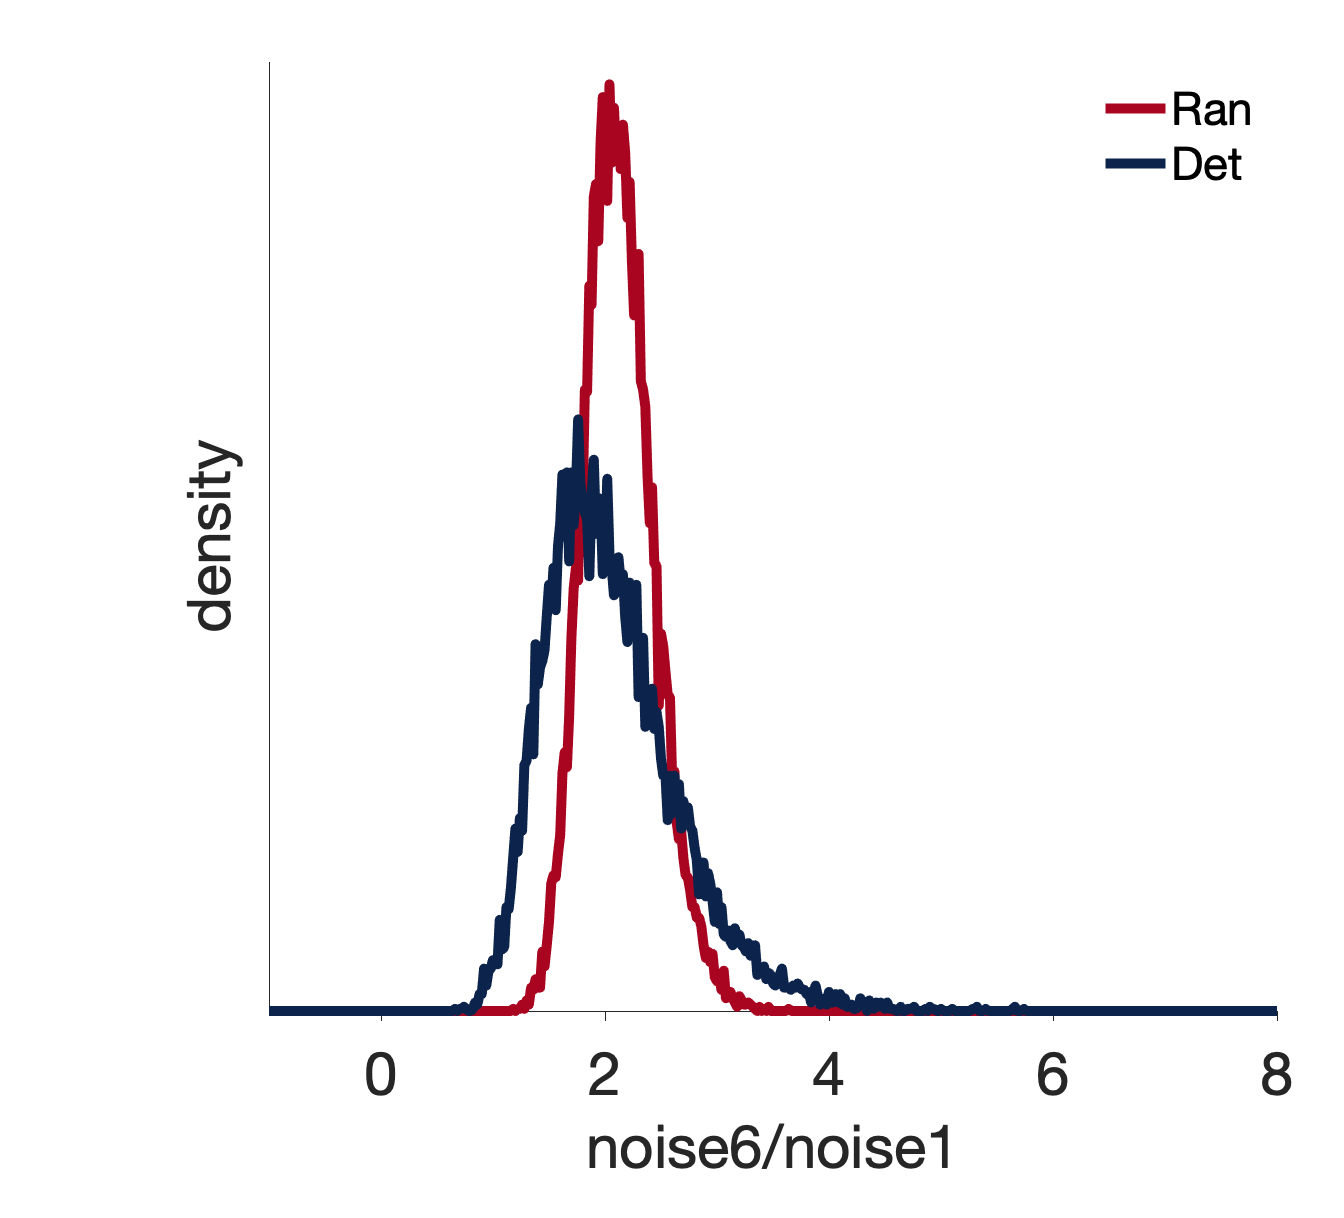
\includegraphics[width=0.6\textwidth]{figures/RanDetNoise_ratio1.png}
			\caption{Model based analysis showing the posterior distributions over the ratio of the group-level mean of the standard deviations of  random and deterministic noise between horizon 6 and horizon 1 respectivelly. The ratio in the standard deviations of noise between horizon 6 and horizon 1 is similar for random and deterministic noise.}
			\label{fig:ratio}
		\end{center}
	\end{figure}

	
	%\begin{figure}[H]
	%	\begin{center}
%			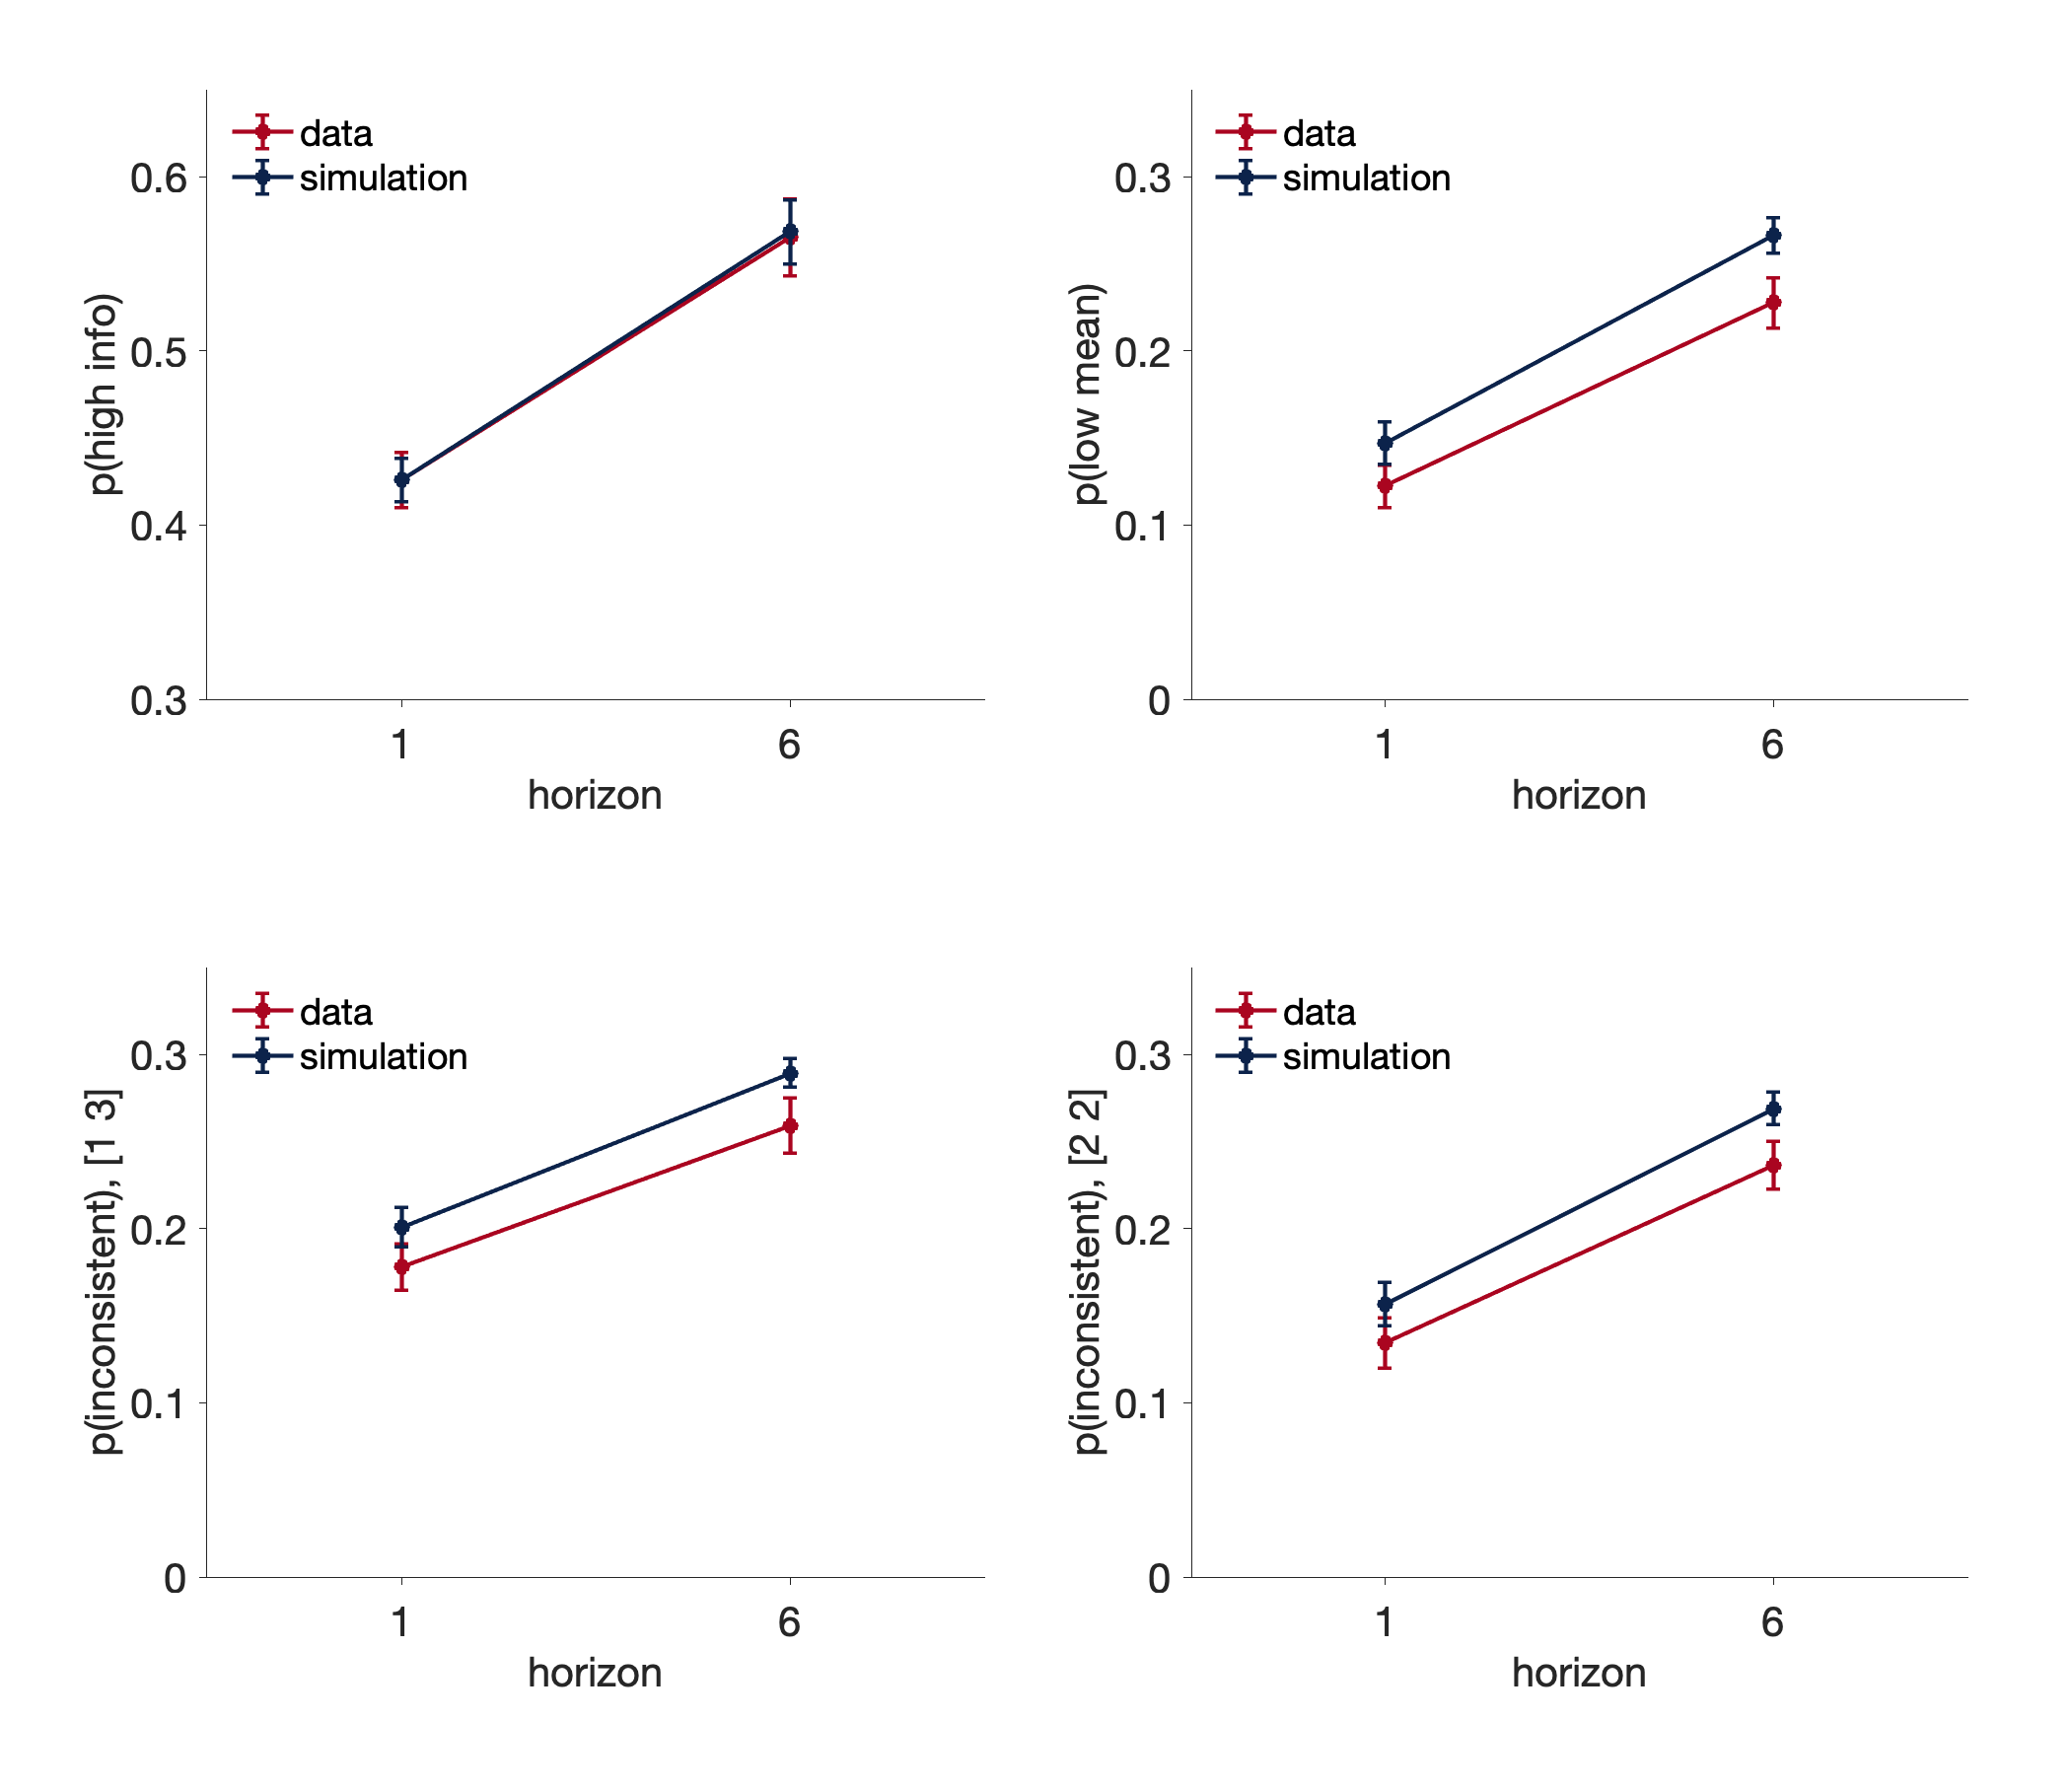
\includegraphics[width=1\textwidth]{figures/pinconsistent_4panel_age_acchance_2noisemodelA_2noisemodelA.png}
%			\caption{}
%			\label{fig:mb2}
%		\end{center}
%	\end{figure}
	
	\subsubsection*{Posterior predictive checks}
	\begin{figure}[hp]
		\begin{center}
			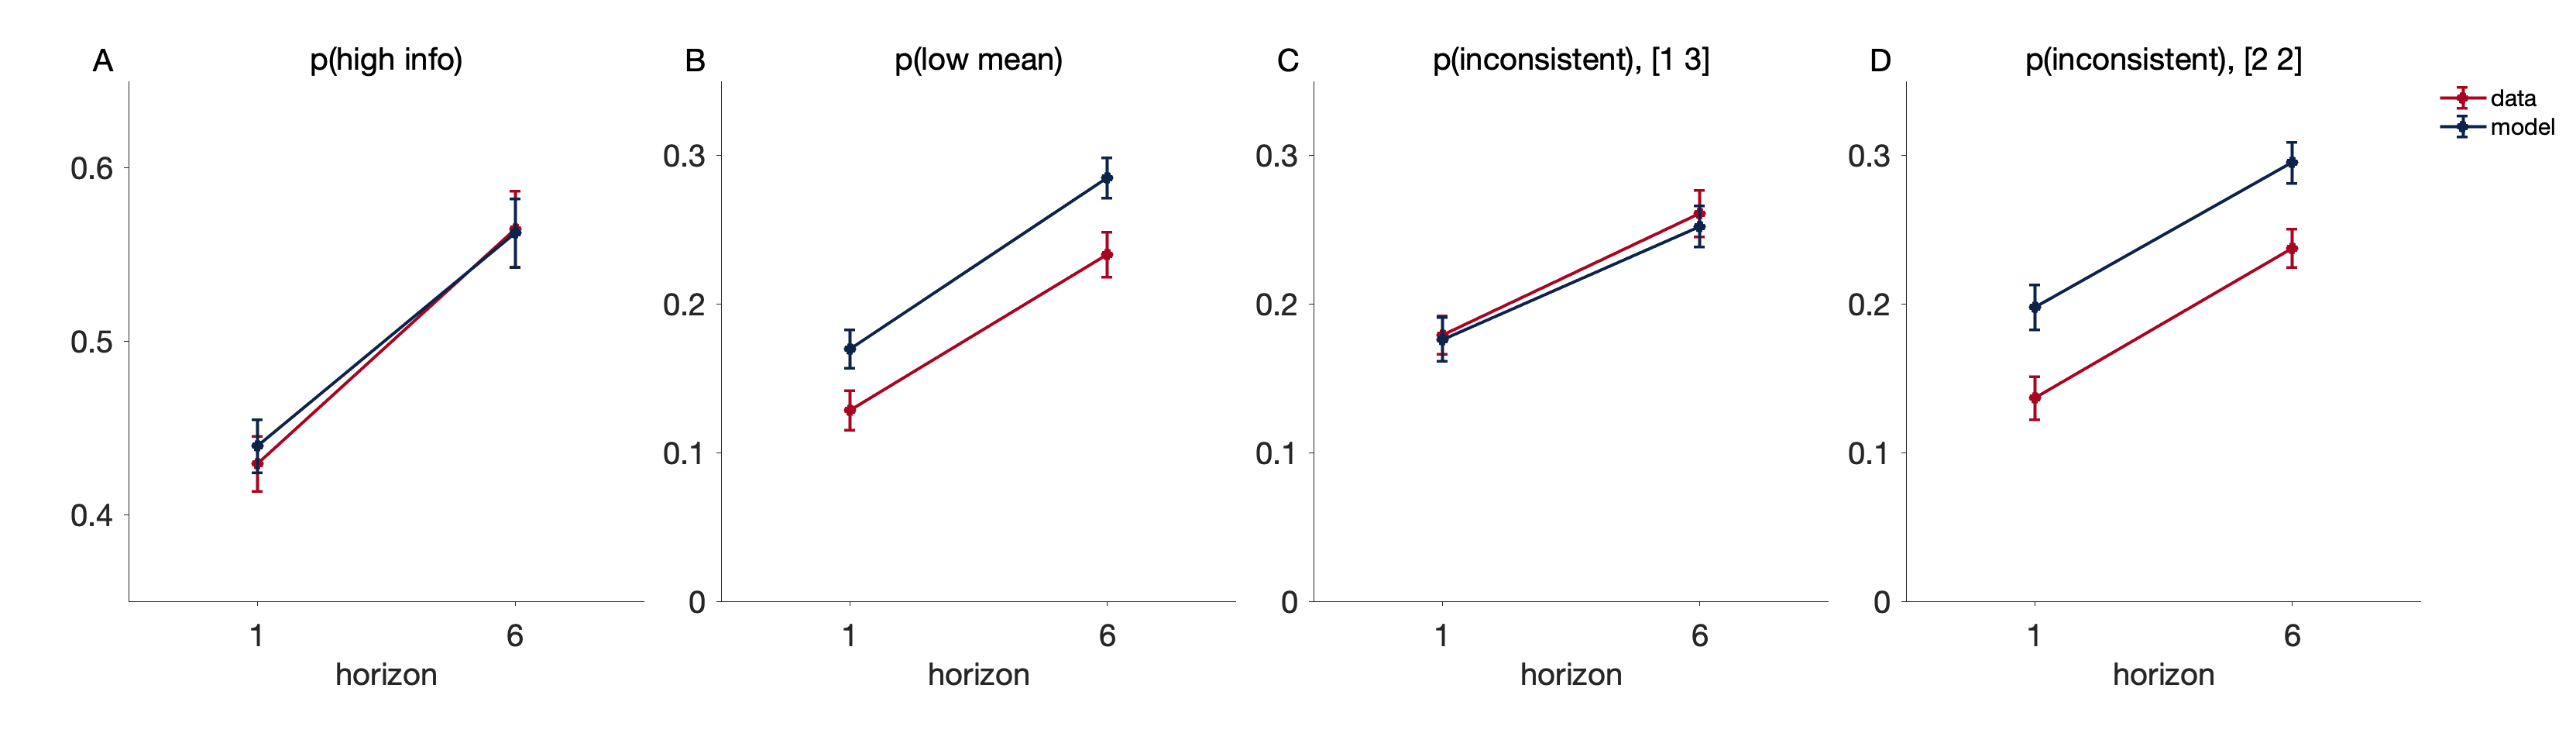
\includegraphics[width=1\textwidth]{figures/pinconsistent_6panel_age_acchance.png}
			\caption{
			% BOB SAYS: KEEP THE TOP LINE OF THIS FIGURE FOR THE MAIN PAPER AND MOVE THE FULL FIGURE TO SUPPLEMENTARY MATERIAL TO FIT DESCRIPTION IN TEXT.  
			% ALSO MAKE THE FOLLOWING CHANGES: THIS FIGURE NEEDS A LEGEND IN TOP RIGHT TO SAY WHICH LINE IS MODEL AND WHICH IS NOT.  I WOULD ALSO USE TEXTBOXES (in Matlab annotation('textbox', [0 0 1 1], 'string', 'hi') will get you started) TO DESCRIBE THE MODELS RATHER THAN LABELLING MODEL A ETC ... COULD EVEN HAVE SOME FORM OF TABLE 1 ON THE LEFT HAND SIDE - SO A COLUMN FOR DETERMINISTIC NOISE AND A COLUMN FOR RANDOM NOISE.
			Our model accounts for all qualitative patterns of the data, namely, p(high info) and p(low mean) increase as a function of horizon, p(inconsistent) increases as a function of horizon for both [1 3] and [2 2] conditions and lies between the pure random and pure deterministic noise prediction.}
			\label{fig:mb3}
		\end{center}
	\end{figure}
	
	In addition to fitting the model to behavior, it is also important to check whether the model captures the qualitative patterns of the data \citep{Wilson2019} --- specifically how p(high info), p(low mean) and p(inconsistent) change with horizon.
	
	To perform this `posterior predictive check,' we created a set of simulated data by taking the subject-level parameters from the hierarchical Bayesian fits and having the model play the same sequence of games as seen by the subjects. We then applied the same model-free analysis as described in the previous sections to this simulated data set and compared the model's behavior to that of participants. As shown in Figure  \ref{fig:mb3}, the model can account for all qualitative patterns in the data --- the increase in p(high info), p(low mean), and p(inconsistent) with horizon, and that p(inconsistent) is in between pure random and pure deterministic noise.  The quantitative agreement is almost perfect for p(high info), but the model seems to systematically underestimate p(low mean) and p(inconsistent), although the discrepancy is small (underestimating p(low mean) by 0.047 or 27.30\%, and p(inconsistent) by 0.027 or 14.27\%).
	
	To check whether all aspects of the model were necessary to reproduce the qualitative pattern of findings, we also built and fit five additional versions of the model.  These models varied whether deterministic and random noise are present or not and whether either types of noise is dependent on horizon. As shown in Supplementary Figure S5, only one of these models, where random noise is horizon dependent but deterministic noise is not, can capture the full qualitative pattern of responding (Note model F does not capture that  p(inconsistent) is between pure random and deterministic?). However, the quantitative fit to the data is not as good (Supplementary Figure S5).
	
	
	%The previous section suggests that behavioral variability in random exploration can be at least partially explained by deterministic processing of the stimulus. 
	
	%dominated by random noise. To test this more explicitly, we build a series of models in which different assumptions are made regarding the presence and absence of both types of noise and whether each type of noise if exists is horizon dependent (See Table \ref{tab:models}). In model A-D, we assumed the existence of both random and deterministic noise, in model A and B, random noise is assumed to be horizon-dependent, whereas in model A and C, deterministic noise is assumed to be horizon dependent. In model E, we assumed no random noise. In model F, we assumed no deterministic noise. 
		
	%To evaluate and compare between models, we simulated choice behavior by taking the subject-level parameters from the Hierarchical Bayesian fits. The same model-free analysis as described in the previous session is applied to all 6 sets of simulated data for the 6 models respectively. (See Figure  \ref{fig:mb3}). 
	
	%The original measure of random exploration, p(low mean), as used in \cite{wilson2014} can be explained by having deterministic noise alone (Figure \ref{fig:mb3}, Panel E2) or having random noise alone (Figure \ref{fig:mb3}, Panel F2). That participants qualitatively exploit the high-mean option less and choose the low-mean option more in horizon 6, can be explained by having both pure deterministic noise and pure random noise, as long as noise is horizon dependent. If both deterministic and random noise are assumed to be the same for both horizons (Figure \ref{fig:mb3}, Panel D), p(low mean) becomes completely flat and no horizon dependent random exploration is observed.
	
	%On the other hand, by looking at the percentage of inconsistent choices in the repeated pair of game, p(inconsistent), external noise alone can not account for behavior any more (Figure \ref{fig:mb3}, Panel E3, E4). Moreover, model C and D are disqualified that the increase of choice inconsistency with horizon can only be qualitatively accounted for when random noise is horizon-dependent (Figure \ref{fig:mb3}, Panel A, B, F).
	
	%Among the models A, B and F, where random noise is horizon dependent, model A provides the best quantitative fit. If there is no deterministic noise (Model F), then we overestimate the level of choice inconsistency in both horizons by a constant. In addition, horizon dependent deterministic noise gives slightly better model fits than if deterministic noise is assumed to be the same in both horizons. Overall, these model simulations confirmed that the horizon dependence of random noise is the main source of random exploration.
	
	
	\section*{Discussion}
	
	% BOB SAYS: CAN YOU TRY TO REFRAME THIS AROUND THE DETERMINISTIC STORY
	
	
	In this paper, we investigated whether random exploration is really random. That is, to what extent is it driven deterministically by aspects of the stimulus we have previously ignored when measuring `decision noise'.  Using a version of the Horizon Task with repeated games, we found evidence that at least some of the noise in random exploration could be explained by such `deterministic noise.' In particular, we found that deterministic noise accounted for XXX\% of the overall variability in people's behavior and increased with horizon - a hallmark of an exploratory process. This suggests that at least some of the apparent randomness in random exploration is not random at all.
	
	%SO WHERE DOES THIS LEAVE RANDOMNESS IN RANDOM EXPLORATION?  WELL, THE REMAINING 75\% OF THE NOISE COULD BE RANDOM OR IT COULD BE DETERMINISTIC BECAUSE WE CAN'T CONTROL EVERYTHING. 
	So where does this leave randomness in random exploration? Well, the remaining XXX \% of the noise could be random or it could be deterministic because we can't control everything. In particular, while we controlled many aspects of the stimulus across repeated games (e.g. the outcomes and the order of the forced trials), we could not perfectly control {\it all} stimuli the participant received, which would vary, for example, based on exactly what they were looking at or whether they were scratching their nose. Thus conceptually, our estimate of deterministic noise is a lower bound. Conversely, our estimate of random noise is an upper bound as these `missing' sources of deterministic noise would be interpreted as random noise in our model. In addition, our estimation method also systematically underestimate deterministic noise (part of the deterministic noise will show up as random noise in model fitting, see Supplementary figure SX), so methodologically our model also provides a lower bound of deterministic noise and an upper bound on random noise. Although there is still a considerable window for truly stochastic processes in the brain to be driving random exploration, our results suggest that at least some of the randomness is driven by a deterministic process instead.
	
	%Given that there is still a considerable window for truly stochastic processes in the brain to be driving random exploration, 
	%Taken at face value, the horizon-dependent increase in random noise is consistent with the idea that random exploration is driven by intrinsic variability in the brain. This is in line with work in the bird song literature in which variability during song learning has been tied to neural variability arising from specific areas of the brain \citep{songbird1, songbird2}. In addition, this work is consistent with a recent report from \cite{ebitz17} in which the behavioral variability of monkeys in an `explore' state was also tied to random rather than deterministic sources of noise. 
	
	%Whether such a noise-controlling area exists in the human brain is less well established, but one candidate theory \citep{aj2005} suggests that norepinephrine (NE) from the locus coeruleus may play a role in modulating random levels of noise. Indeed, changes in the NE system have been associated with changes behavioral variability in both humans and other animals in a variety of tasks \citep{eeKarpova14, eeKeung18}.  In addition there is some evidence that NE plays a direct role in random exploration \citep{eeWarren17}, although this finding is complicated by other work showing no effect of NE drugs on exploration \citep{jepma2012, nieuwenhuis05}
	
	%More generally, our finding that random noise dominates behavioral variability over deterministic noise, is consistent with findings of \cite{drugowitsch16}. In particular these authors show that randomness in behavior arises from imperfections in mental inference, that happen inside the brain, rather than in peripheral processes such as sensory processing and response selection. This suggests that most noise in behavior is generated randomly and that this may arise from  computational errors in computing the correct strategy. In the context of the Horizon Task, such computational errors would likely be larger  in the long horizon condition as the correct course of action in these cases is much harder to compute.
	
	
	%USE TEXT FROM THIS PARAGRAPH IN THE `WHERE DOES THIS LEAVE RANDOMNESS PARAGRAPH' 
	%Perhaps the main limitation of this work is that we cannot say whether the remaining XXX\% of the noise is deterministic or is actually random.	
	
	Regardless of whether the remaining XXX\% is deterministic or random, the fact that thee horizon change in the two noises are proportional to each other suggests a possible mechanism for random exploration, Specifically, a reduction in the strength with which reward drives the choice. In particular, in our analysis we excluded a scalar on $Delta R$, if we include that then we get
	
	%REGARDLESS OF WHETHER THE REMAINING 75\% IS RANDOM OR NOT, THE FACT THAT THE HORIZON CHANGE IN THE TWO NOISES ARE PROPORTIONAL TO EACH OTHER SUGGESTS A POSSIBLE MECHANISM FOR RANDOM EXPLORATION.  SPECIFICALLY, A REDUCTION IN THE STRENGTH WITH WHICH REWARD DRIVES THE CHOICE.  IN PARTICULAR, IN OUR ANALYSIS WE EXCLUDED A SCALAR ON $\Delta R$.  IF WE INCLUDE THAT THEN WE GET
	\begin{equation}
	    \Delta Q = \beta \Delta R + A \Delta I + b + n_{det} + n_{ran}
	\end{equation}
	
	A decrease in $beta$ here would be equivalent to an increase in variance of both deterministic and random noise. Such reduced coding of reward would be consistent with \cite{ebitz17} (NEED CHECK).
	%A DECREASE IN $\beta$ HERE WOULD BE EQUIVALENT TO AN INCREASE IN VARIANCE OF BOTH DETERMINISTIC AND RANDOM NOISE.  MAKES THE PREDICTION THAT SPATIAL BIAS SHOULD ALSO CHANGE IN PROPORTION (CHECK THIS!).
	
	%SUCH REDUCED CODING OF REWARD WOULD BE CONSISTENT WITH EBITZ (I THINK).
	
	
	%Despite this, it seems hard to imagine that these additional noise sources could be enough to account for the large differences between random and deterministic noise that we found in Figure \ref{fig:mb1}, where random noise is 2-3 times the size of deterministic noise.  
	
	

	
	\bibliographystyle{plainnat}
	%\bibliographystyle{unsrt}
	\bibliography{Refs/refs}
	
	% add the Bibliography to the Table of Contents
	\cleardoublepage
	\ifdefined\phantomsection
	\phantomsection  % makes hyperref recognize this section properly for pdf link
	\else
	\fi
	\addcontentsline{toc}{chapter}{Bibliography}
	


\end{document}
